\documentclass[]{article}
\usepackage{lmodern}
\usepackage{amssymb,amsmath}
\usepackage{ifxetex,ifluatex}
\usepackage{fixltx2e} % provides \textsubscript
\ifnum 0\ifxetex 1\fi\ifluatex 1\fi=0 % if pdftex
  \usepackage[T1]{fontenc}
  \usepackage[utf8]{inputenc}
\else % if luatex or xelatex
  \ifxetex
    \usepackage{mathspec}
  \else
    \usepackage{fontspec}
  \fi
  \defaultfontfeatures{Ligatures=TeX,Scale=MatchLowercase}
\fi
% use upquote if available, for straight quotes in verbatim environments
\IfFileExists{upquote.sty}{\usepackage{upquote}}{}
% use microtype if available
\IfFileExists{microtype.sty}{%
\usepackage{microtype}
\UseMicrotypeSet[protrusion]{basicmath} % disable protrusion for tt fonts
}{}
\usepackage[margin=1in]{geometry}
\usepackage{hyperref}
\hypersetup{unicode=true,
            pdftitle={princ\_math},
            pdfborder={0 0 0},
            breaklinks=true}
\urlstyle{same}  % don't use monospace font for urls
\usepackage{graphicx,grffile}
\makeatletter
\def\maxwidth{\ifdim\Gin@nat@width>\linewidth\linewidth\else\Gin@nat@width\fi}
\def\maxheight{\ifdim\Gin@nat@height>\textheight\textheight\else\Gin@nat@height\fi}
\makeatother
% Scale images if necessary, so that they will not overflow the page
% margins by default, and it is still possible to overwrite the defaults
% using explicit options in \includegraphics[width, height, ...]{}
\setkeys{Gin}{width=\maxwidth,height=\maxheight,keepaspectratio}
\IfFileExists{parskip.sty}{%
\usepackage{parskip}
}{% else
\setlength{\parindent}{0pt}
\setlength{\parskip}{6pt plus 2pt minus 1pt}
}
\setlength{\emergencystretch}{3em}  % prevent overfull lines
\providecommand{\tightlist}{%
  \setlength{\itemsep}{0pt}\setlength{\parskip}{0pt}}
\setcounter{secnumdepth}{0}
% Redefines (sub)paragraphs to behave more like sections
\ifx\paragraph\undefined\else
\let\oldparagraph\paragraph
\renewcommand{\paragraph}[1]{\oldparagraph{#1}\mbox{}}
\fi
\ifx\subparagraph\undefined\else
\let\oldsubparagraph\subparagraph
\renewcommand{\subparagraph}[1]{\oldsubparagraph{#1}\mbox{}}
\fi

%%% Use protect on footnotes to avoid problems with footnotes in titles
\let\rmarkdownfootnote\footnote%
\def\footnote{\protect\rmarkdownfootnote}

%%% Change title format to be more compact
\usepackage{titling}

% Create subtitle command for use in maketitle
\newcommand{\subtitle}[1]{
  \posttitle{
    \begin{center}\large#1\end{center}
    }
}

\setlength{\droptitle}{-2em}

  \title{princ\_math}
    \pretitle{\vspace{\droptitle}\centering\huge}
  \posttitle{\par}
    \author{}
    \preauthor{}\postauthor{}
    \date{}
    \predate{}\postdate{}
  

\begin{document}
\maketitle

\hypertarget{mathematical-statistical-and-dynamics-principles}{%
\section{Mathematical, Statistical and Dynamics
Principles}\label{mathematical-statistical-and-dynamics-principles}}

\hypertarget{difference-equations}{%
\subsection{Difference Equations}\label{difference-equations}}

In mathematics, a basic representation of a process over time is a
difference equation:

\begin{equation}
\label{basicD}
y_{t} = y_{t - 1}
\end{equation}

\noindent where \(y_{t}\) represents \(y\) now and \(y_{t-1}\) is the
variable at the prior time point. Here, the value of \(y\) is the same
at each \(t\), and the emergent behavior would be a flat line across
time. In systems theory terms, there would be no trend.

Although equation \ref{basicD} seems simple, it introduces a fundamental
concept in dynamics: memory. The variable now depends on where it was in
the past. It is constrained, there are boundaries on where it can go.

As we add terms to this basic difference equation the behavior of the
variable becomes more complex. Adding a forcing constant, \emph{c} in
equation \ref{basicD} produces positive or negative trend depending on
whether \emph{c} is, respectively, positive or negative. For example,
the following equation:

\begin{equation}
\begin{split}
\label{diffC}
y_{t} &= y_{t-1} + c \\ 
c &= -4
\end{split}
\end{equation}

\noindent produces a line that decreases by four units at each time
point.

The next level of complexity comes from autoregressive terms, which
represent the extent to which the variable relates to itself over time.
Here:

\begin{equation}
\begin{split}
\label{diffA}
y_{t} &= a y_{t-1} \\ 
a &= 0.5
\end{split}
\end{equation}

\noindent the variable is described over time but it does not retain the
same value at each \(t\). Instead, the variable is \emph{similar} over
time and the autoregressive term, \(a\), describes the extent of that
similarity. In equation \ref{diffA}, \(a\) is 0.5, meaning that the
relationship between the variable now and itself at the next time point
will be 0.5.

There are fundamental behaviors of dynamic variables based on their
autoregressive terms, and these are shown in figure \ref{dynamics_plot}.
The top row of figure \ref{dynamics_plot} shows the trajectory of
variables with autoregressive terms that are greater than one in
absolute value. These large terms produce explosive behavior --
exponential growth when \(a\) is positive and oscillating chaos when
\(a\) is negative. When the autoregressive term falls between zero and
one in absolute value, conversely, the variable converges to equilibrium
-- shown in the bottom two panels. Either the variable oscillates at a
decreasing rate until it reaches equilibrium (when \(a\) is negative) or
it converges there smoothly (when \(a\) is positive).

\begin{verbatim}
## -- Attaching packages ---------------------------------------------------------------------------------------------------------- tidyverse 1.2.1 --
\end{verbatim}

\begin{verbatim}
## √ ggplot2 3.0.0     √ purrr   0.2.5
## √ tibble  1.4.2     √ dplyr   0.7.6
## √ tidyr   0.8.1     √ stringr 1.3.1
## √ readr   1.1.1     √ forcats 0.3.0
\end{verbatim}

\begin{verbatim}
## -- Conflicts ------------------------------------------------------------------------------------------------------------- tidyverse_conflicts() --
## x dplyr::filter() masks stats::filter()
## x dplyr::lag()    masks stats::lag()
\end{verbatim}

\begin{figure}
\centering
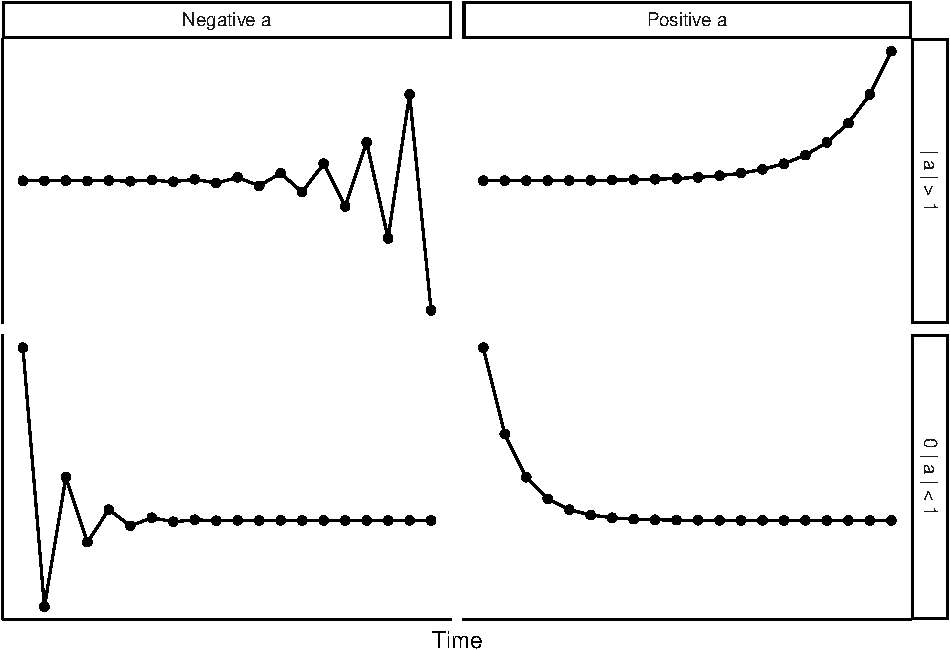
\includegraphics{princ_math_files/figure-latex/unnamed-chunk-1-1.pdf}
\caption{something here\label{dynamics_plot}}
\end{figure}

\begin{center}

---------------

Insert Figure \ref{dynamics_plot} Here

---------------

\end{center}

\hypertarget{equilibrium}{%
\subsection{Equilibrium}\label{equilibrium}}

Equilibrium, then, describes the state of a variable that no longer
changes unless disturbed by an outside force. It can also be used to
describe multiple variable systems. In these contexts, equilibrium again
means that the state remains constant unless disturbed by an outside
force, but here it refers to the state of the entire system (i.e., all
of the variables). In \emph{static} equalibriums, the system has reached
a point of stability with no change, whereas \emph{dynamic} equilibrium
refers to systems with changes and fluctuations but no net change. That
is, the variables fluctuate across time in periodic ways but the general
state of the system does not diverge so as to change the behavior of the
entire system.

Predator-prey relationships are a typical example of a system in dynamic
equilibrium. For example, consider a predator-prey relationship between
bobcats and rabbits. As the rabbit population increases, the amount of
available food for the bobcats goes up. Over time, this raises the
population of the bobcats as well. Now with a greater bobcat population,
the rabbit population decreases because more are being killed. Over
time, this reduction in food opportunity decreases the bobcat
population. This back and forth oscillating pattern between variables
describes a dynamic equilibrium. The variables change and there may be
random disturbances to the system across time, but the net dynamics of
the system remain stable.

Our route so far has been deterministic. That is, the mathematical
representations do not contain error. Conveying that the underlying
process -- the data generating mechanism -- contains error presents us
with a host of additional principles.

\hypertarget{stochastics}{%
\subsection{Stochastics}\label{stochastics}}

Stochastics, stated simply, refers to processes with error. Consider our
simple difference equation from above, adding an error component
produces:

\begin{equation}
\label{diffE}
y_{t} = a y_{t-1} + c + e_{t}
\end{equation}

\noindent where all terms are defined above but \(e_{t}\) represents an
error component that is incorporated into \(y\) at each time point.
Errors cause \(y\) to be higher or lower at specific points in time than
we would have expected given a deterministic process. For example, at
time \(t\) the error might push \(y\) to a higher value, and at
\(t + 1\) to a lower value. Errors are therefore said to be random
because we cannot predict their value at any specific \(t\). In
aggregation (i.e., averaged across time), however, positive errors
cancel negative errors, and large errors are less likely than small
errors. Any time we have an accumulation of random error we get a normal
distribution {[}@mcelreath{]}. In stochastic systems, therefore, the
errors are said to be distributed \(N(0, 1)\) -- that is, random and
unpredictable at any specific \(t\) but distributed with certain
constraints across time.

It can also be helpful to think about what error is not. Anything that
is systematic, predictable, or common (using those in layman's terms)
cannot be error.

\hypertarget{white-noise-and-random-walks}{%
\subsection{White Noise and Random
Walks}\label{white-noise-and-random-walks}}

There are two fundamental stochastic processes: white noise and random
walks. White noise is a process that only has error. Setting \emph{c}
and \emph{a} to zero in equation \ref{diffE} produces a white noise
process.

\begin{equation}
\begin{split}
\label{whitenoise}
y_{t} &= a y_{t-1} + c + e_{t} \\ 
a &= 0
c &= 0
\end{split}
\end{equation}

\noindent Here, all we have is error over time. Panel ``A'' of figure
\ref{noise} shows the behavior of a white noise process over time.
Random walks are similar, but \emph{a} is now equal to one.

\begin{equation}
\begin{split}
\label{rw}
y_{t} &= a y_{t-1} + c + e_{t} \\ 
a &= 1
c &= 0
\end{split}
\end{equation}

\noindent This representation is also an error process, but there is
self-similarity across time. Panel ``B'' of figure \ref{noise} presents
a random walk. Although random walks can sometimes appear to be moving
in a systematic direction, ultimately their behavior is unpreditable:
they could go up or down at any moment.

Random walks and white noise are error processes over time. White noise
processes fluctuate randomly, whereas random walks fluctuate randomly
while retaining some self-similarity through time. These two principles
are the null hypotheses of time-series analysis in econometrics -- where
the first task in a longitudinal study is to demonstrate that you are
investigating something that is not a random walk or white noise.

\begin{verbatim}
## Warning in plot.formula(rnorm(10, 0, 1) ~ rnorm(10, 0, 1)): the formula
## 'rnorm(10, 0, 1) ~ rnorm(10, 0, 1)' is treated as 'rnorm(10, 0, 1) ~ 1'
\end{verbatim}

\begin{figure}
\centering
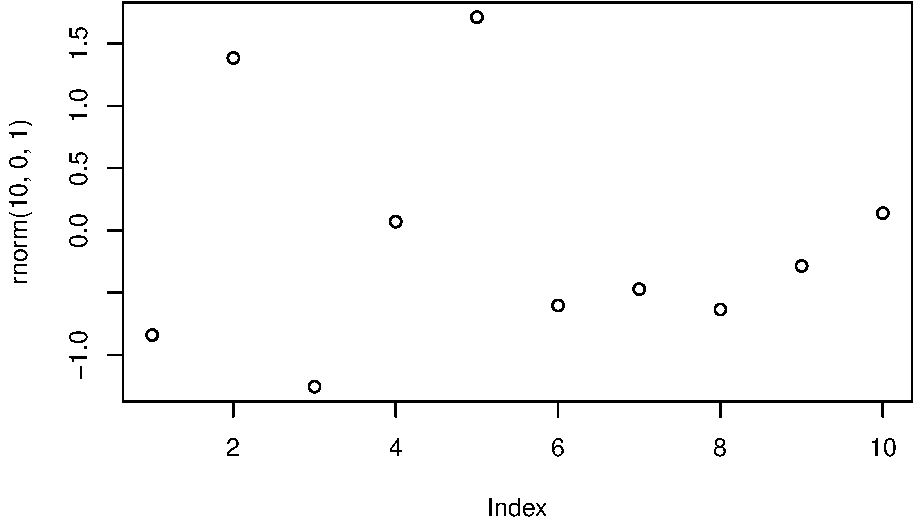
\includegraphics{princ_math_files/figure-latex/unnamed-chunk-2-1.pdf}
\caption{another\label{noise}}
\end{figure}

\hypertarget{stationarity}{%
\subsection{Stationarity}\label{stationarity}}

Modeling techniques make assumptions about the data generating process
they attempt to capture, and a key assumption in dynamic models is
stationarity, or the stability of properties in a time series.
Stationarity subsumes two requirements: mean stationarity, which refers
to a series with a constant mean, and variance stationary, which refers
to a series with a constant variance. Almost all dynamic models used in
the organizational literature are stationary models and assume the data
they model are realizations of a stationary process. In simple terms,
this means that we expect the properties (mean and variance) of a time
series at time \(t\) to be the same at time \(t+1\).

In general, we are interested in the relationships between one or more
time series or panel trajectories. Acknowleding stationarity is critical
for analyzing these relationships because two series that are
non-stationary will be related regardless of the data generating process
{[}@kuljanin2010; @braun2010{]}. That is, two (or more) independent
variables that share no causal relationship will appear related in the
observed data when they have trend. The first step in a dynamic
analysis, then, is to check whether there is evidence of trend (i.e.,
non-stationarity).

The most common method for checking stationarity is the Dickey-Fuller
(ADF) test {[}@dickey1979{]} in which the null hypothesis is that the
time series contains a time-\emph{dependent} error term. If the series
is stationary, it will contain a time-\emph{invariant} error term and
thus the ADF significance test will be rejected. This test was designed
in the econometrics literature where single time-series are more
prevalent than panel data (repeated measures designs with many
\emph{N}), but equivalent tests are now available for data structures
more consistent with those found in the organizational literature.

Complete explanations of stationarity tests for both time-series and
panel data are available in @jebb2017 and @braun2010. Because our
interest here, consistent with the organizational literature, is on
panel data and not single time-series relationships we use a panel
version of the Dickey-Fuller test.

\hypertarget{cointegration}{%
\subsection{Cointegration}\label{cointegration}}

In the current paper we assessed stationarity before moving to formal
data modeling because Granger and Newbold {[}-@granger1974{]}
demonstrated that regressions between independent non-stationary series
will likely produce significant coefficient estimates and large \(R^2\)
values. Analyzing series with independent (i.e., unrelated/not causal)
trends, random walks, or uneven variance across time, therefore, will
likely result in spurious inference. It is also possible, however, that
two non-stationary processes are related. We then need a way to assess
that relationship without biasing our results in the manner presented by
Granger and Newbold (1974). In a later paper, Granger
{[}-@granger1986{]} showed that, under very specific circumstances, we
can garner evidence for a relationship between two non-stationary
series. Formally, two series, \(x\) and \(y\) are said to be
cointegrated if 1) both are integrated of the same order, \(I(d)\), and
2) they share a linear combination that is \(I(0)\). In other words,
there is a linear combination of \(x\) and \(y\) that is stationary
(requirement \#2) and they both require the same number of steps to make
them stationary (requirement \#1).

The basis for cointegration is simple: do we have evidence for a
relationship between series in a situation where we know spurious
relationships are likely (i.e., non-stationarity)? Implementing
cointegration techniques, however, is much more difficult. The analyst
needs to be sensitive to the type of non-stationarity present in the
series: trends or random walks. A random walk is defined as

\begin{equation}
y_{t} = 1*y_{(t-1)} + e_{t}
\end{equation}

\noindent where the variable is exactly what it was at the prior time
point but also accumulates error across time. These series may increase,
decrease, or change directions at any instant. A series with trend is
simply one that increases or decreases over time. Again, the steps
required to demonstrate cointegration change if the analyst is dealing
with trends or random walks. The analysis also changes if the variables
are single-units or panels. Cointegration was developed for time-series
data but panel techniques are also available now {[}@kao1999{]}. At this
point we recommend ensuring data are stationary. Cointegration merits
another paper entirely.

\hypertarget{granger-causality-and-directionality}{%
\subsection{Granger Causality and
Directionality}\label{granger-causality-and-directionality}}

X granger causes Y if Y can be better predicted by the histories of both
X and Y than the history of Y alone. If lagged values of X help predict
current values of Y in a forecast formed from lagged values of both X
and Y, then X is said to Granger cause Y. We implement this notion by
regressing eggs on lagged eggs and lagged chickens; if the coefficients
on lagged chickens are significant as a group, then chickens cause eggs.
A symetric regression tests the reverse causality. We perform the
Granger causality tests using one to four lags. The number of lags in
each equation is the same for eggs and chickens. To conclude that one of
the two ``came first,'' we must find unidirectional causality from one
to the other. In other words, we must reject the noncausality of the one
to the other and at the same time fail to reject the noncausality of the
other to the one. If either both cause each other or neigher causes the
other, the question will remain unanswered. Results reject that eggs do
not Granger cause chickens. They provide no such reject of the
hypothesis that chickens do not Granger cause eggs. Therefore, we
conclude that eggs cause chickens. A better phrasing might be
``temporally related'' (Granger \& Newbold, p.~225) -- Thurman and
Fisher 1988 call it temporally ordered.

\hypertarget{diffusion}{%
\subsection{Diffusion}\label{diffusion}}

\hypertarget{damping}{%
\subsection{Damping}\label{damping}}

\hypertarget{markov-process}{%
\subsection{Markov Process}\label{markov-process}}


\end{document}
